\chapter{Results}\label{ch:results}


\section{General features of the simulated data}\label{sec:general-features-of-the-simulated-data}

The NMM is configured to simulate data with a step-size of $1 ms$, yielding a $1000 Hz$ signal.
In its initial state, the system reacts with high-amplitude oscillations to the "disturbance" of the random input.
However, the signal usually stabilizes quickly and exhibits the expected behaviour.
Thus, the first few seconds (stabilization-time varies with parameterization) of simulated data
are always discarded before further analysis.
When generating data continuously (without re-initialization of the state-variables),
this problem only occurs once in the very beginning.
Changing system parameters abruptly during simulation can also result in disturbances and destabilize the
signal.

\begin{figure}[H]
    \centering
    \begin{tikzpicture}
        \pgfplotsset{
        %% Axis
            scale only axis,
            width=0.4\linewidth,
            height=4cm,
            every axis/.append style={
                line width=1pt,
                tick style={line width=0.8pt},
                %   grid style={dashed, black!20},
                %  grid=major,
            },
%               %% X-Axis
            xmin=-0.1,
            xmax=7,
        }
        \begin{groupplot}
            [
            group style={
                group size=2 by 1,
                vertical sep=2mm,
                horizontal sep=15mm,
                xlabels at=edge bottom,
                xticklabels at=edge bottom,
            },
            yticklabel style={
                /pgf/number format/fixed,
                /pgf/number format/precision=2
            },
            legend style={nodes={scale=0.8, transform shape}, thin},
            legend image post style={scale=0},
            xlabel=$s$,
            ]
            \nextgroupplot[ylabel=$mV$]
            \addplot [line width=.5pt,solid, cyan] table[x=x,y=y ,col sep=comma]{data/methodology/uncut.csv};
            \legend{\textbf{A} uncut data};
            \nextgroupplot[xmin=3.0]
            \addplot [line width=.5pt,solid, cyan] table[x=x,y=y ,col sep=comma]{data/methodology/uncut.csv};
            \legend{\textbf{B} cut data};

        \end{groupplot}
    \end{tikzpicture}

    \caption{
        \textbf{Processing of simulated data.}\\
        Simple Jansen-Rit Model with $C=135$. \\
        \textbf{A \& B:} removing initially unstable signal by cutting off the first $3s$ of the data.
    }
    \label{fig:initial_oscilations}
\end{figure}


\section{Visualization}\label{sec:visualization}




\begin{figure}[H]
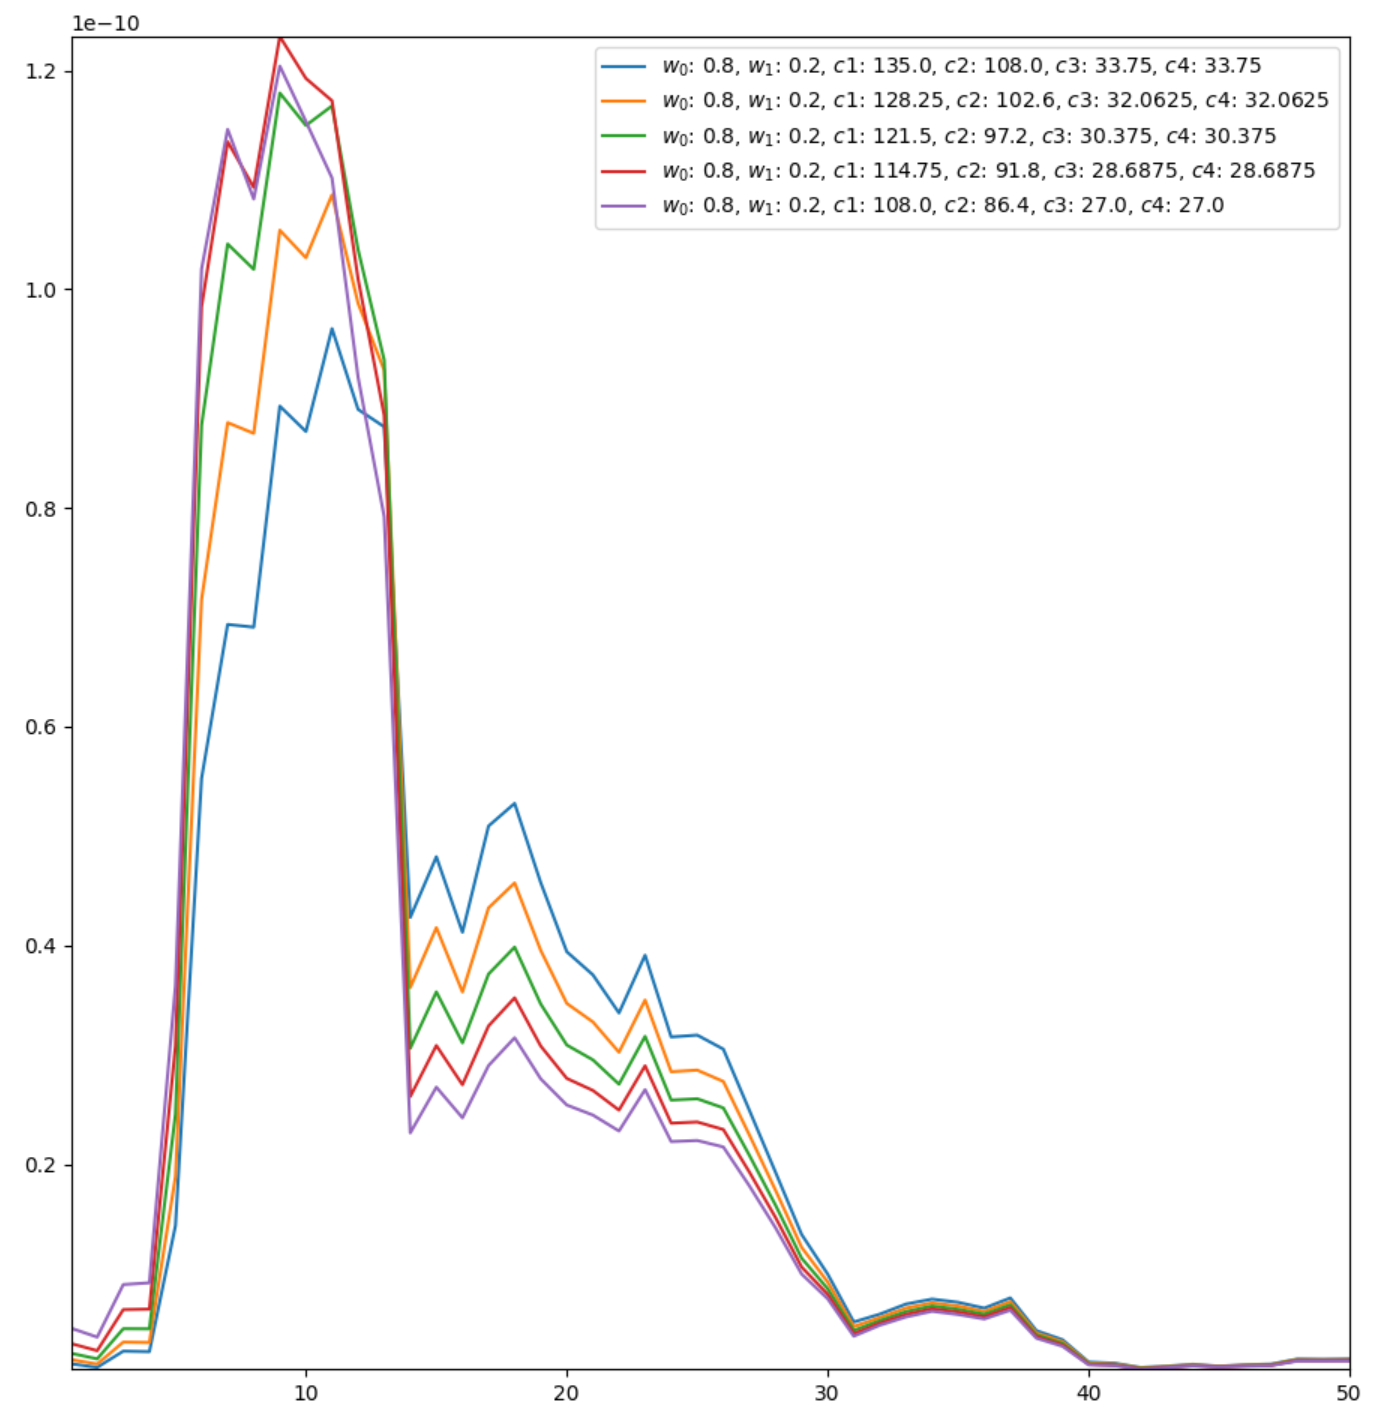
\includegraphics[width=15cm]{Figures/temp_sim_results}
\caption{\textbf{Power Spectral Density of Simulation Results:} Reduction of the connectivity parameter $C$
    from $135$ to $108$ shows a tendency of reducing the strength of the frequency-bands above 12--14Hz,
    while increasing it below that value - especially around 8--12Hz.}
\label{fig:sim_results1}
\end{figure}

\todo{objective description of simulation results}